\chapter{Introduction}
\label{chapter:Introduction}



%background: automated driving / driver assistance
%TU9
%thesis proposal description
%computer vision
%need for high performance computing on both gpu and fpga
%currently not possible to transfer data directly from gpu to fpga in opencl
%=focus of this thesis


\section{Background}

%TODO blablabla

%memory wall?
%instead parallelism
%GPGPU mainstream since CUDA
%FPGAs starting to be used in this area as well
Steadily rising processor clock frequencies were the driving force behind computational performance gains throughout the previous century.
However, this frequency scaling came to an end around the year 2005 due to its side effect of very high power consumption, known as the power wall.
This has forced computer science to develop new techniques to maintain the increase of computational speed.
The focus of research has shifted towards parallelism, which enables computations to be performed simultaneously instead of sequentially.
Previously employed mainly in supercomputers, parallel computing has become mainstream with the development of parallel processor architectures like multi-core CPUs, GPUs and FPGAs.

%With the power wall becoming a larger problem, more power-efficient devices....


%heterogenous computing!!

%became mainstream since multi-core cpus and cuda

%co-processors/accelerators
%opencl
%reconfigurable computing

%Despite being originally developed only for graphics applications, \emph{graphics processing units} (GPUs) are today extensively used for computationally intensive general purpose computing.

GPUs and FPGAs are typically used as accelerators or co-processors in addition to a CPU.
Such a \emph{heterogeneous} computing system can combine the advantages of its individual components.
The CPU is best suited for sequential and control tasks, whereas data-parallel computations are best to be performed on the GPU or FPGA accelerators.
Exploiting the differences among the different accelerator architectures can result in even higher performance gains.
FPGAs are hard to beat in bit shifting operations, integer arithmetic and interfacing peripheral devices (such as cameras) but are deficient on floating point operations for which GPUs can accommodate \cite{chimera}.
%The accelerators themselves also
%Splitting the work accross the accelerators can 


%applications: computer vision, scientific comutations
Typical applications for heterogeneous computing systems include computer vision, physical simulations or scientific visualization.
Specifically a CPU-GPU-FPGA system has been used at the TU Munich for lane detection in the context of automated driving \cite{lanedetection}.



\section{Problem Statement}


%XXX copypasted from wikipedia
% Communication and synchronization between the different subtasks are typically some of the greatest obstacles to getting good parallel program performance.


%an issue with accelerators is the transfer from host to device
%XXX: copypasted from thesis description, rephrase
%A key requirement of such heterogeneous computing system is the ability to
%transfer data between components at high bandwidth and low latency
%transfer delays are always undesired
%bandwidth is often the bottleneck

High bandwidth and low latency data transfer between individual components are vital for the performance of a heterogeneous computing system.
Methods for the communication between the CPU and the accelerator devices are usually provided by the corresponding vendors.
Communication between accelerators from different vendors however, has to take the cumbersome and slow approach of a round trip via the CPU.


%TODO:expected results
%evaluate

%diagram from/like bittner?


\begin{center}
\begin{figure}[ht]
\hspace{1.3cm}
\begin{minipage}[b]{0.35\linewidth}
\centering
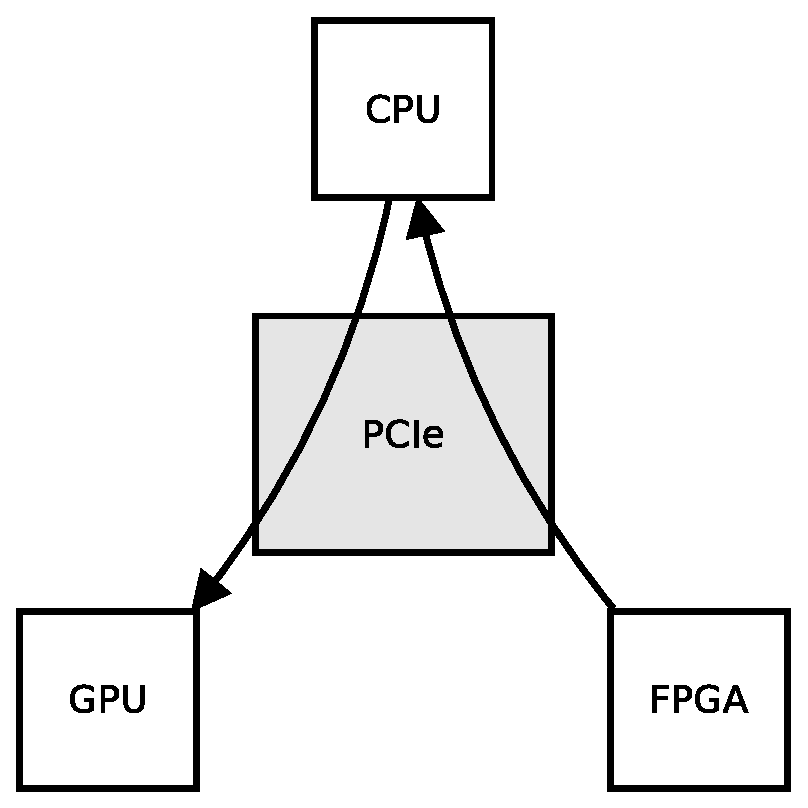
\includegraphics[width=\textwidth]{images/indirect.eps}
\caption{\emph{Indirect} GPU-FPGA transfer}
\label{fig:indirect}
\end{minipage}
\hspace{1.8cm}
\begin{minipage}[b]{0.35\linewidth}
\centering
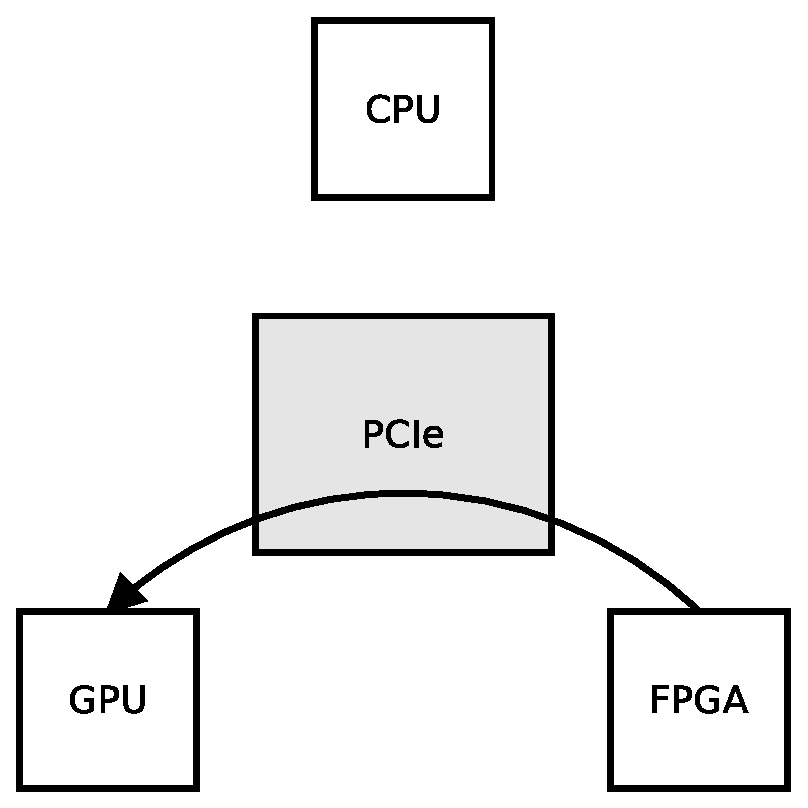
\includegraphics[width=\textwidth]{images/direct.eps}
\caption{\emph{Direct} GPU-FPGA transfer}
\label{fig:direct}
\end{minipage}
\end{figure}
\end{center}




The goal of this thesis is to enable the still missing direct link between the GPU and the FPGA.
A holistic framework for direct GPU-FPGA transfers based on the OpenCL computing platform should be developed.
Specifically, a NVIDIA graphics card and an Altera FPGA board shall communicate directly over the PCIe bus with minimal coordination by the CPU.
A significant bandwidth improvement compared to the indirect method is to be expected.



This thesis is structured as follows:
\begin{itemize}
	
\item Chapter \ref{section:theory} provides a brief overview over the technologies that are required to fully understand the later parts of this thesis.
\item In chapter \ref{section:previouswork} previous developments in this direction are presented. %and what is the difference to this work
\item Chapters \ref{section:icd} and \ref{section:implementation} document the efforts during the actual development of the framework.
\item Chapter \ref{section:concurrent} describes an alternative to the direct GPU-FPGA communication that may be suitable in many cases.
\item The evaluation of the developed methods and a comparison with the previous approaches are presented in chapter \ref{sec:results}.
\item Lastly, chapter \ref{section:conclusions} discusses the results and suggests further developments that could not be finished during this thesis.

\end{itemize}





